
In order to generate a final system, i.e., obtain all the source files of a custom embedded system it is imperative the use of the \textbf{\textit{EL} Framework.} This tool, developed by the entire Embedded System class, provides the ability to write a program which models a reference architecture of a particular domain, using the \textbf{\textit{EL} language}. Later, through user (consumer) configurations, the source files for that specif domain are created with personal customization. Since the workflow is much more complex than that, this section describes the process as well as its intrinsic elements and also a user perspective view of the use of the framework.

\subsection{Overview}

The EL Language and the framework were based in a standard \textbf{set of specifications} for the definitions of models, called  \textbf{S}ervice \textbf{C}omponent \textbf{A}rchitecture (\textit{SCA}). The specific domains to be modeled can be seen as a set of \textbf{software components working together}, and so, two things are required: a way to create components and a mechanism for describing how they work together in complete particular domains. 
 
Every \textit{SCA} based application is built from one or more components and their interactions. Those interactions are established by interfaces where components can refer \textbf{services} provided by others. Also, it specifies how those components can be combined into larger structures called \textbf{composites}. Figure \ref{fig:CompositeModel} shows a simple composite composed by two components.

 \begin{figure}[!htb]
\centering
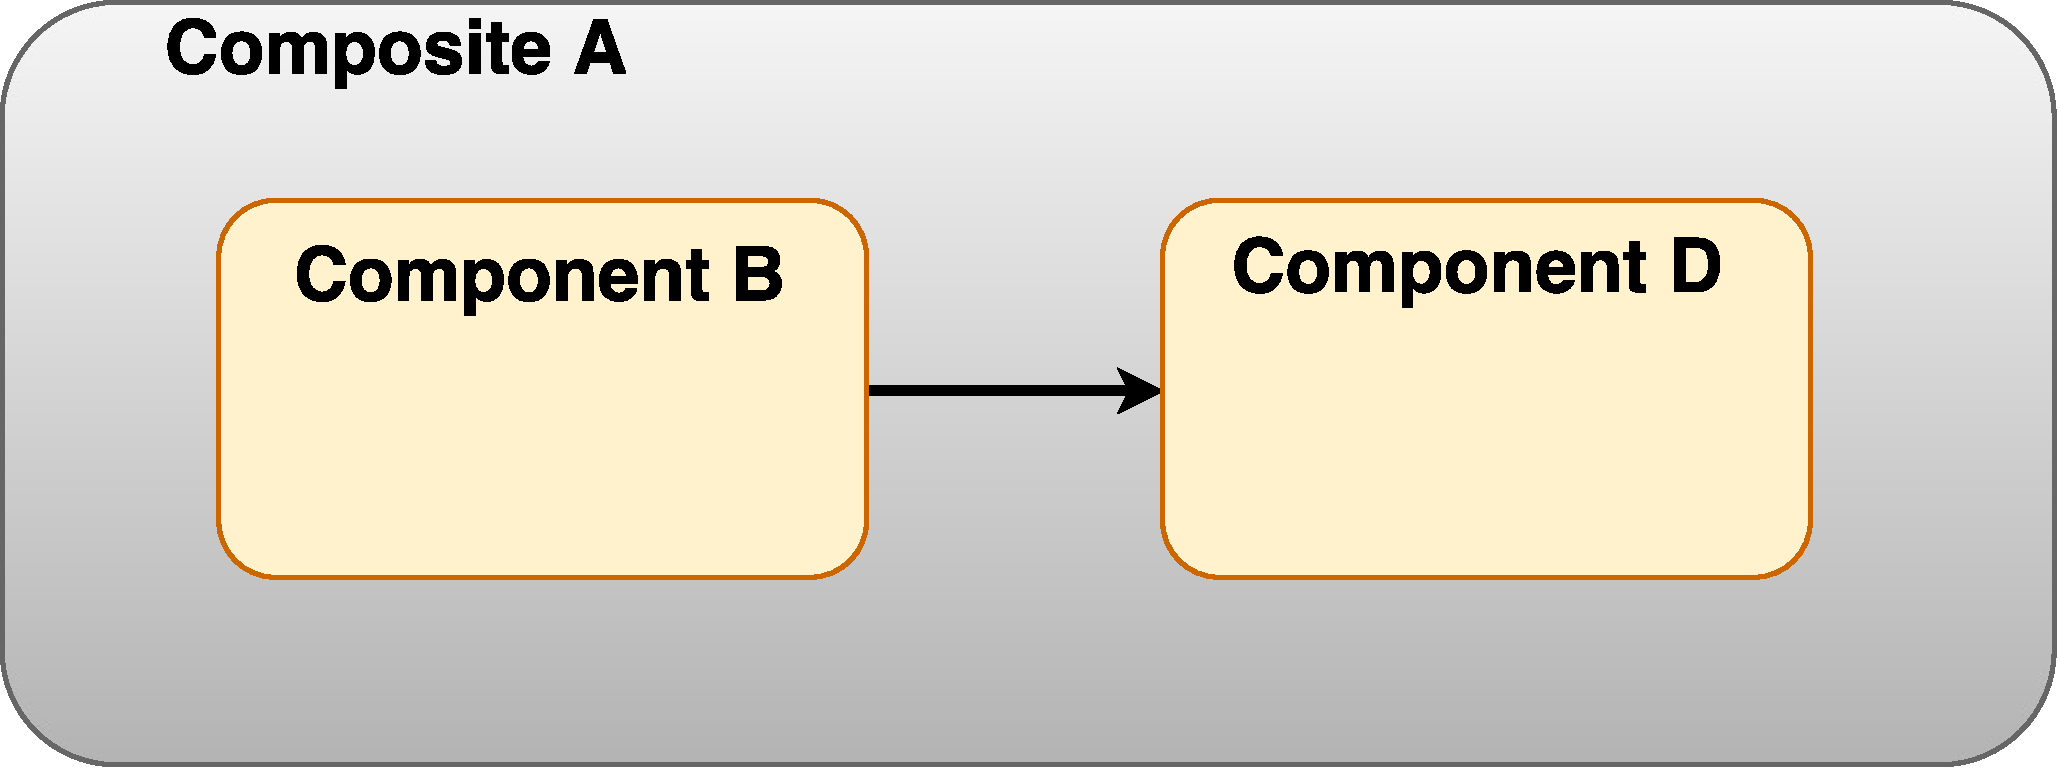
\includegraphics[scale=0.25]{images/CompositeModel}
\caption{Simple Composite.}
\label{fig:CompositeModel} 
\end{figure}
 
A complete application can be constructed from just one composite (figure \ref{fig:CompositeModel}) or through a combination of several different composites (figure \ref{fig:CompositeModel2}). Those are then considerate components if they are integrated in another composite and so on. 
 
\begin{figure}[H]
\centering
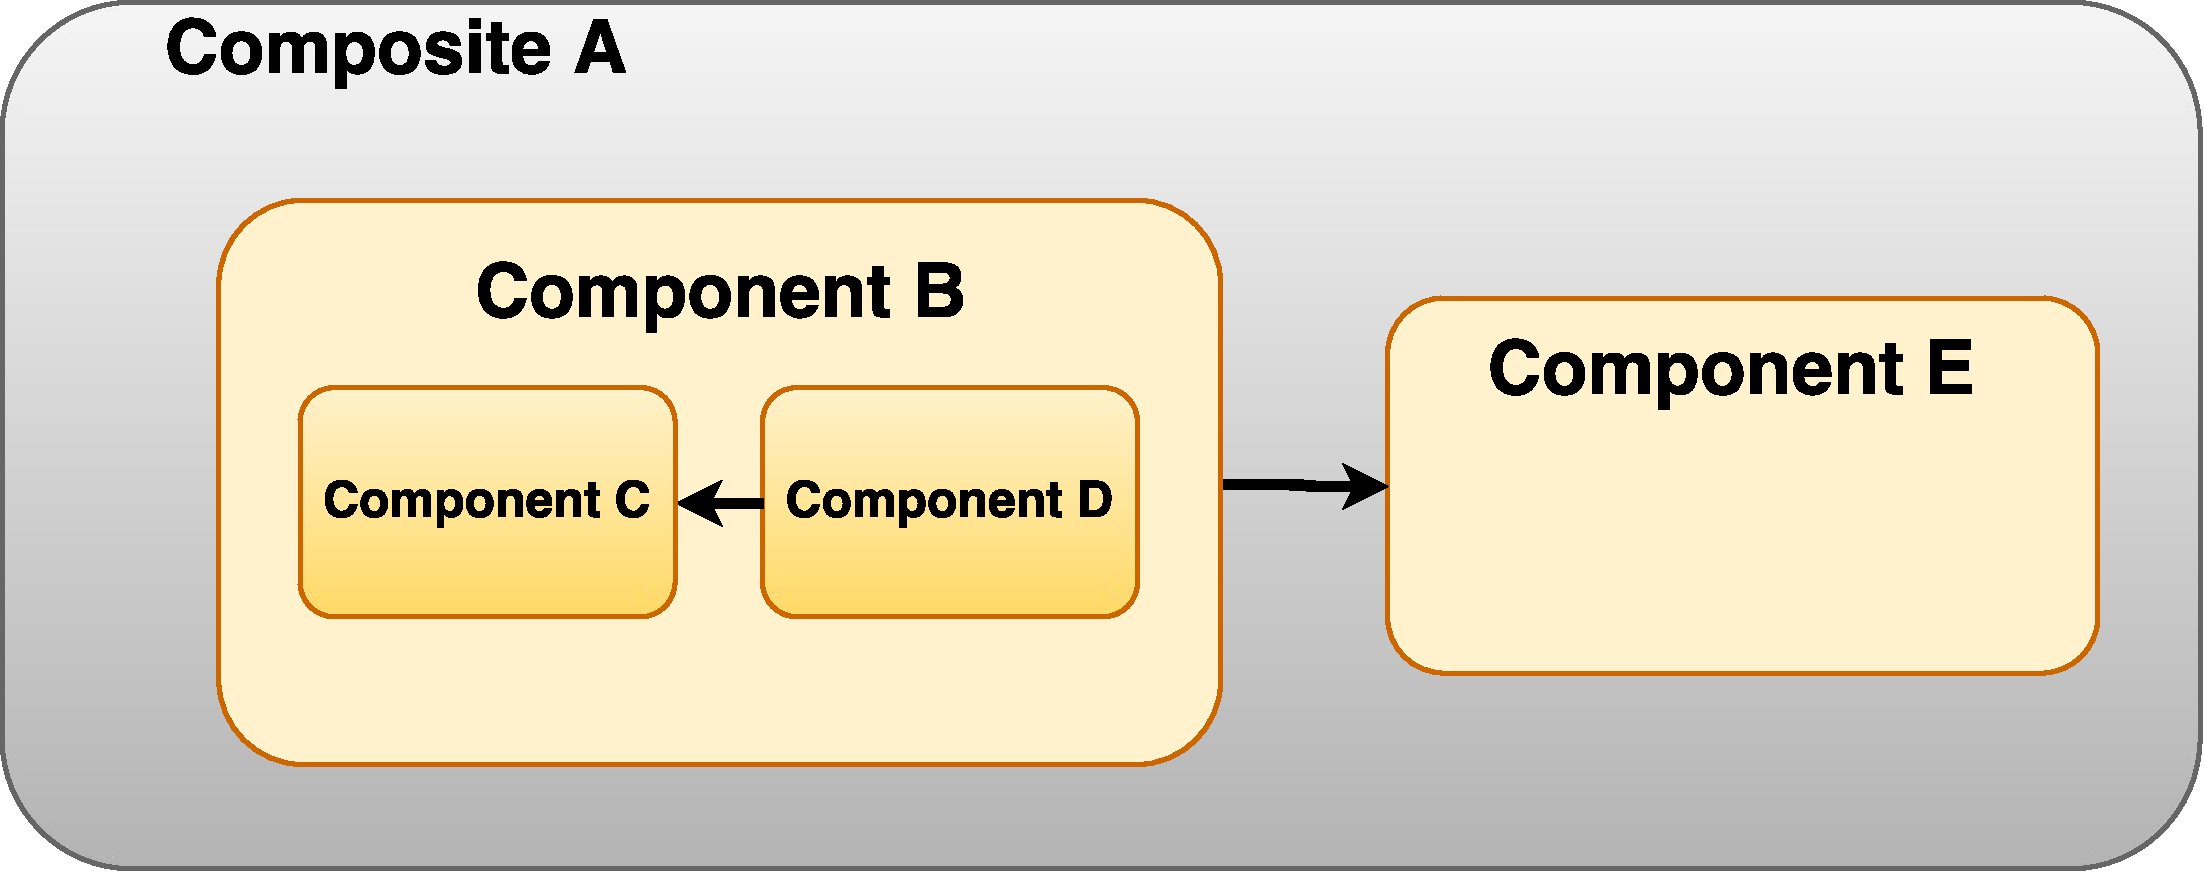
\includegraphics[scale=0.22]{images/CompositeModel2}
\caption{Larger Composite.}
\label{fig:CompositeModel2} 
\end{figure}
 
Components are the atoms from which an \textit{SCA} application is created. Like atoms, \textit{SCA} components behave in consistent ways, and they can be assembled into different configurations. Thus, every component relies on a common set of abstractions, including: \textbf{properties}, \textbf{promotes}, \textbf{services}, \textbf{references} and \textbf{bindings}. \cite{SCA_site} These terms will be recalled later with definitions and respective contextualization with the \textit{EL} Framework. 
 
To sum up, the \textit{SCA} was a reference point for the design of the \textit{EL} framework and for the development of the \textit{EL} language. So, all the conceptual modelization of the particular domains must follow, partly, the \textit{SCA} specifications in order to ensure compatibility with the language, and so, with the framework. In the next sections, it will be covered the full specifications for the definition of the models along with the exhibition of relevant topics related to the \textit{EL} language. Also, the workflow of the EL framework will be illustrated and analyzed aiming the clarification of the process, since the conceptual modelization until the generation of the final source files of a software system.  

\subsection{\textit{EL} Language}

To materialize the conceptual model of a particular domain, an \textit{.el} file must be created. Basically, that process consists in coding the model using the \textit{EL} language. In this section, it will be presented an overview of the language's syntax and semantics as well as its keywords. For consolidation of ideas, along with the explanations, examples of a conceptual model and respective \textit{.el} file will be shown.

\subsubsection{Semantics Overview}

As mentioned, the \textit{SCA} was used as reference point for the development of the language. Its specifications for \textbf{component, properties, references, services, promotes} and \textbf{bindings} were maintained. However, an extension were made to include \textbf{assignments}, as will be presented next. A simple conceptual model (figure \ref{fig:ModelExample}) was created to show how these attributes shall be used.

\begin{figure}[H]
\centering
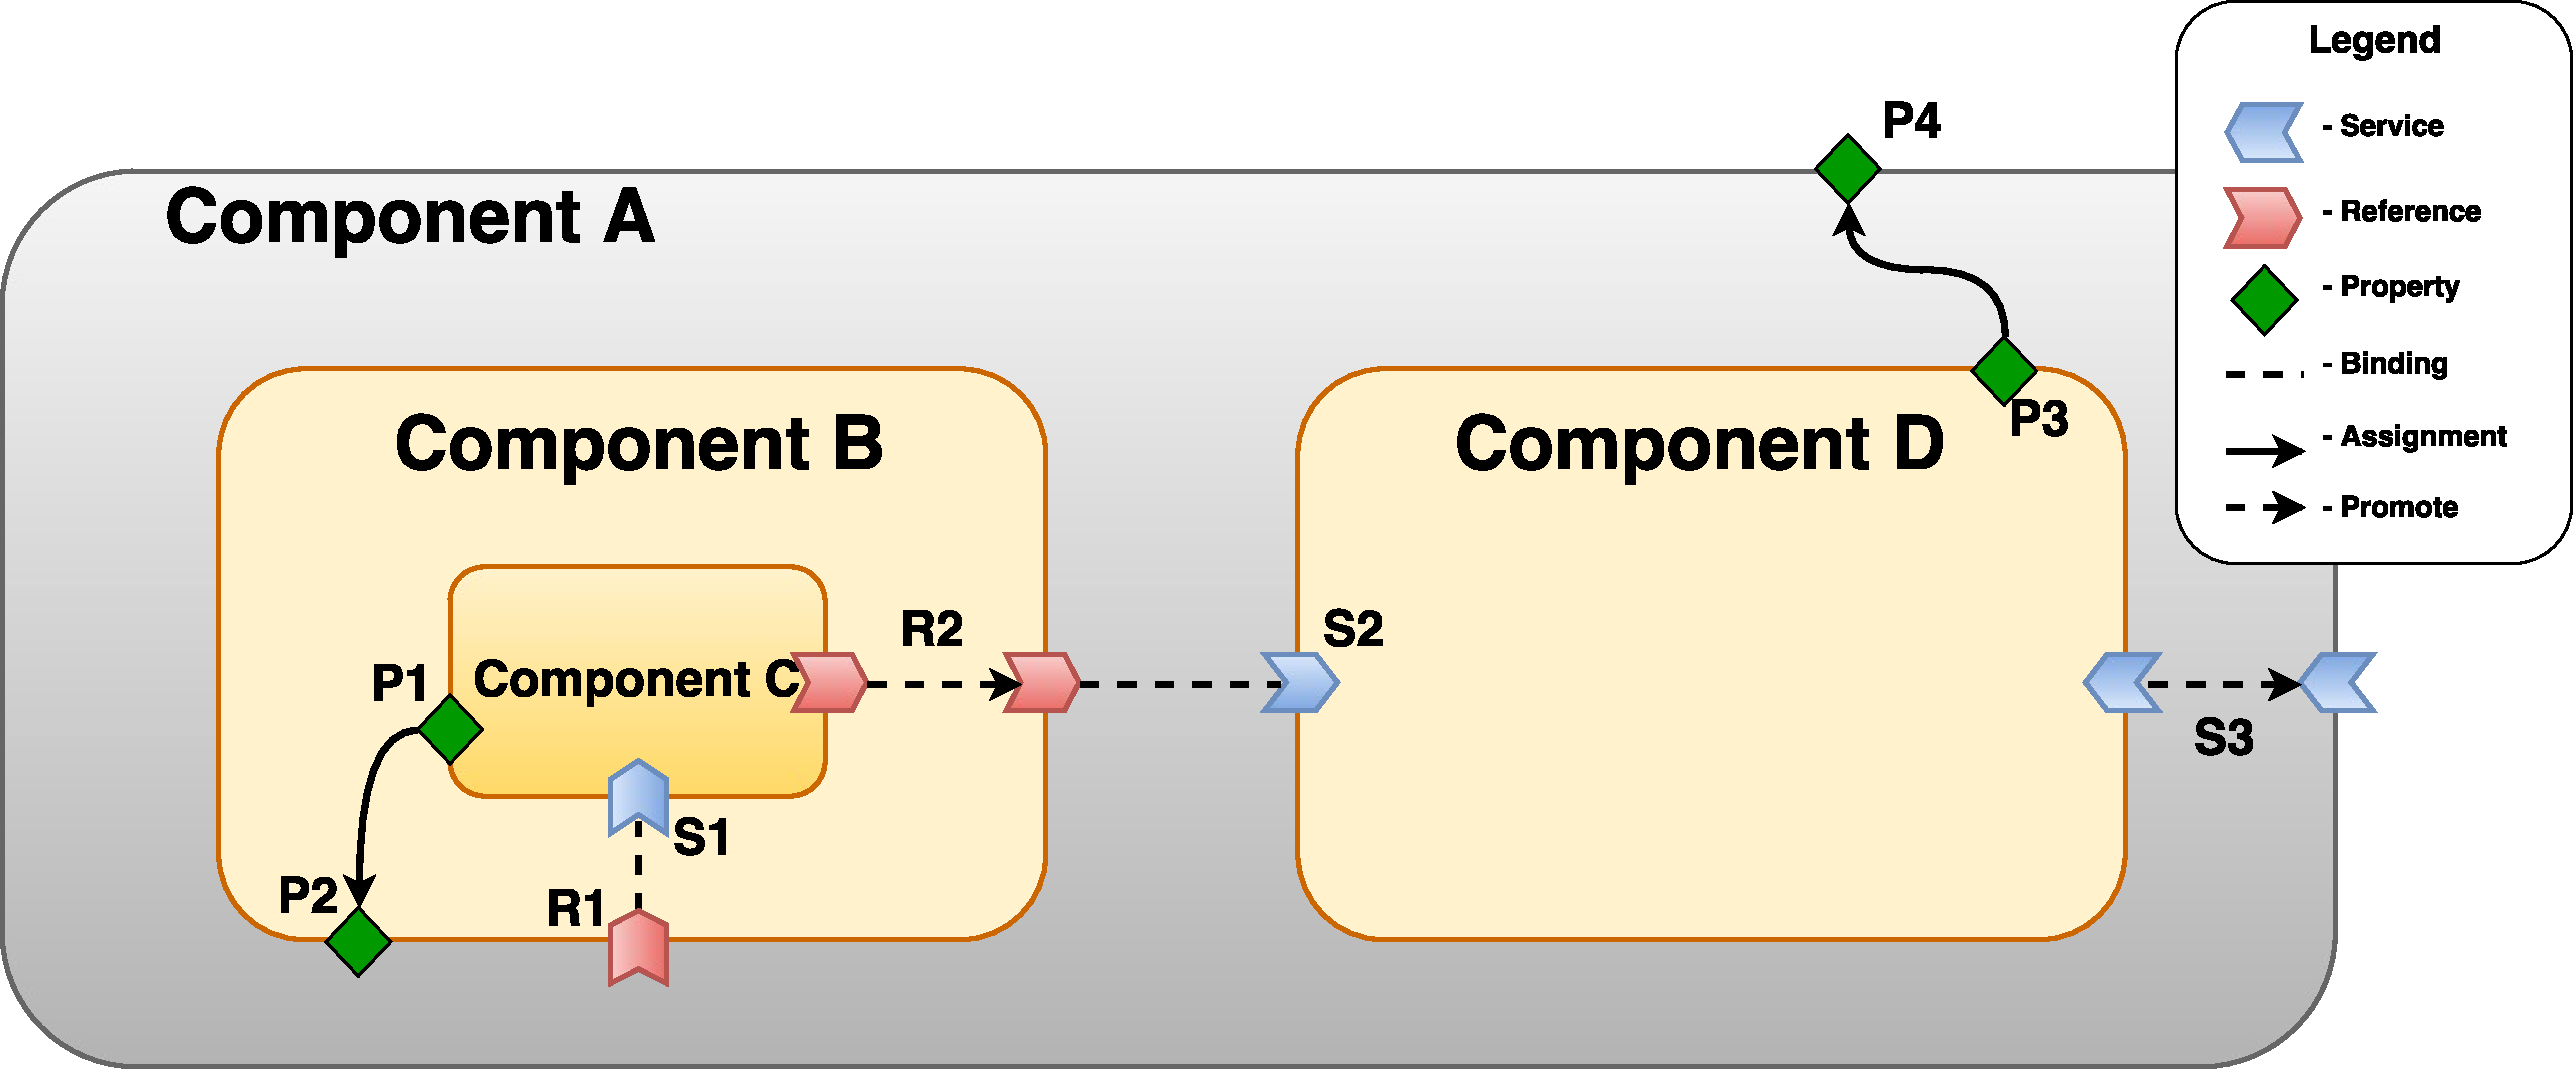
\includegraphics[scale=0.25]{images/ModelExample}
\caption{Simple Conceptual Model.}
\label{fig:ModelExample} 
\end{figure}

\subsubsubsection*{Component}
A top level \textbf{component} can wrap another components, which then can be considered as \textbf{subcomponents}. This way, the top level can access all the properties, references and services of its subcomponents. That is illustrated in figure \ref{fig:ModelExample} where \textit{C} is a subcomponent of \textit{B}, and \textit{B} and \textit{D} are subcomponents of \textit{A}.

\subsubsubsection*{Property and Assignments}
A component's \textbf{property} is an attribute whose value is configurable by the user. During the explanation of the framework's workflow it will become clear the role of the properties. The \textbf{assignments} allows the creation of \textbf{dependencies} between properties. In the simple model, it is visible the dependency between property \textit{P1} and property \textit{P2} and the relation between property \textit{P3} and \textit{P4}.

\subsubsubsection*{References, Services and Bindings}
As referred, one of the main characteristics of the pattern used for the modelization of systems is the existence of interaction between components described as components that need services from other components. This translates in \textbf{references} to \textbf{services}. Figure \ref{fig:ModelExample} shows an example of this type of relation: \textit{B} has a reference \textit{R1} bound to a service \textit{S1} of its subcomponent \textit{C}. This \textbf{binding} is established given the existence of \textbf{interfaces} between them. 

\subsubsubsection*{Promotes}
A \textbf{Promote} allows bindings between references and services that are not accessible through the components scope. This means that when references and services are promoted, their visibility is extended to upper components. In the presented conceptual model, the reference \textit{R2} form \textit{C} is promoted by \textit{B}, therefore, \textit{A} can bind it to the service \textit{S2} provided by \textit{D}.


\subsubsection{Syntax Overview}

In the previous topic, an overview of  \textit{EL} language semantics was made by using a simple conceptual model. Now, this model will be transposed into an ".el" file in order to see the syntax of the language. 

\subsubsubsection*{Language}

The first definition that must be done is the \textbf{language} of the original source files. This entity is necessary for semantics checks since the language of a component must be the same as its subcomponents. It defines the attribute \textbf{annotation} which contains the characters that identifies the location for replacements. 
\begin{lstlisting}[language=EL, caption={Language definition in .el file}, label=lst:lang]
      language C_language
      {	
      				annotation: "##"	
      }    
\end{lstlisting}

\subsubsubsection*{Interface}

Before the definition of the components and its bindings, the \textbf{interfaces} must be created in order to define the services that are provided by the components. Those interfaces can be filled with a list of attributes representing the possible methods/functions implemented in the source files. Listing \ref{lst:inter} shows the interfaces declared for the example in study.

\begin{lstlisting} [language=EL, caption=Interface definition in .el file, label=lst:inter]
      interface interface1{
          function1
      }
      interface interface2{
          function2_1  
          function2_2
      }
      interface interface3{
          function3
      }
\end{lstlisting}


\subsubsubsection*{Component}    

At last, it comes the declaration of the entity component, shown in listing \ref{lst:comp}. The example shows the definition of the component \textit{A}, defined as the top level component of the architecture. 

\begin{lstlisting} [language=EL, caption=Component definition in .el file, label=lst:comp]
      import "language.el"
      import "interface.el"
      import "B.el"
      import "D.el"

      compile A

      component A (C_language)
      {
          subcomponents:
              B b
              D d
          properties:
              string P4
              
          bind b.R2_promoted to d.S2
          promote service d.S3 as S3_promoted
          P4 = d.P3
      }
\end{lstlisting}

The definition of a component goes through several fields that should be filled (not all mandatory):

\begin{itemize}
\item The component's \textbf{name} (\textit{A}) and the source code \textbf{language} (\textit{C\_language}).
\item The \textbf{subcomponents} section used to declare other components that belongs to it (\textit{B} and \textit{D}).
\item The \textbf{properties} section which contains configurable points for the user (\textit{P4}).
\item The \textbf{bindings} section used to wire \textbf{references} (\textit{b.R2}) from one component to \textbf{services} provided by another (\textbf{d.S2}).
\item The \textbf{promote} section where \textbf{references} (\textit{d.S3}) and \textbf{services} declared in its subcomponents can be promoted and visible with a \textbf{new name} (\textit{S3\_promoted}) in upper components.
\item The \textbf{assignment} section where operation on properties are made (\textit{P4 = d.P3}).
\end{itemize}

The example shows also an important keyword in in the language: \textbf{compile}. This keyword is used to inform the compiler which is the top level components that must be used for the generation of the artifacts of the framework, as it will be shown in the following section.

An additional feature is related with imported files. In order to access entities of the model declared in other files (language, interface, component), it is possible to import those files in the top of the \textit{.el} file (\textbf{import} section).


\subsubsection*{Keywords} 

Table \ref{keywordsTable} shows all keywords defined in the \textit{EL} language. Some were already presented in the previous section. This table was obtained from the manual created for the framework in Embedded Systems' course. 

\begin{table}[H]
	\centering
	\caption{EL keywords.}
	\label{keywordsTable}
    \centerline{
	\begin{tabular}{|l|l|}
		\hline
		%\rowcolor[HTML]{C0C0C0} 
		\textbf{Keywords}        & \textbf{Description}		\\ \hline
		\textcolor{red}{annotation} 				 & Defines the character that limits the annotations	\\ \hline
		\textcolor{red}{as}                       & Renames a promoted reference or service \\ \hline
		\textcolor{red}{bind}                     & Binds a reference to a service  \\ \hline
		\textcolor{red}{bool}                     & Component's property data type   \\ \hline
		\textcolor{red}{compile}					 & Tells to compiler which is the top level component \\ \hline
		\textcolor{red}{component}				 & Defines a component	\\ \hline 
		\textcolor{red}{final}					 & Defines that a component has a concrete elaboration \\ \hline
		\textcolor{red}{import} 				     & Imports the content of the specified file	\\ \hline
		\textcolor{red}{int}                      & Component's property data type   \\ \hline
		\textcolor{red}{interface} 			     & Defines a set of functions used by a service or pointed by a reference \\ \hline
		\textcolor{red}{is}						 & Inherits the specified component \\ \hline
		\textcolor{red}{float}                    & Component's property data type   \\ \hline
		\textcolor{red}{language}				 & Defines a language		\\ \hline
		\textcolor{red}{promote}                  & Promotes a reference or service from a subcomponent to a component \\ \hline
		\textcolor{red}{properties}               & Defines the properties set of a component     \\ \hline
		\textcolor{red}{reference}                & Defines the reference used in a promote or in a bind operation  \\ \hline
		\textcolor{red}{references}               & Defines the references set of a component \\ \hline
		\textcolor{red}{restrict}                 & Restricts the values that a property can take to a user's defined set  \\ \hline
		\textcolor{red}{service}                  & Defines the service used in a promote or in a bind operation \\ \hline
		\textcolor{red}{services}                 & Defines the services set of a component  \\ \hline
		\textcolor{red}{string}                   & Component's property data type \\ \hline
		\textcolor{red}{subcomponents}            & Defines the subcomponents set of a component  \\ \hline
		\textcolor{red}{to}                       & Connects a reference to a service in a bind operation \\ \hline
	\end{tabular} }
\end{table} 



\subsection{\textit{EL} Workflow}

In this section it will be presented the magic that is behind the \textit{EL} framework. This way, it is intended to illustrate the flow of events since the \textbf{creation of the \textit{.el} files} until the \textbf{generation of the final sources}, describe some important steps of that process and also enumerate and explain relevant \textbf{artifacts} related to the all mechanism.

\subsubsection{Artifacts}

There is a set of artifacts involved on the functioning of the framework. Those artifacts are: \textbf{\textit{EL} files}, \textbf{Configuration Files}, \textbf{Source Files}, \textbf{Elaboration Files} and the \textbf{Elaborator}. Each one of them has an important role on the workflow and a brief explanation will be presented next.

\subsubsubsection*{\textit{EL} files} 

The \textit{EL} files were already presented in the previous section. As it known, this set of files are an \textit{EL} representation of the model. They will be interpreted by the compiler in order to generate the correct workflow for the elaboration. The workflow will be given by the
components relations and contents.

\subsubsubsection*{Configuration files}

The configuration files are generated by the compiler and it is created one per component. Being in a XML representation, its purpose is to allow the \textbf{configuration of the component's properties} by the user. These properties may represent configurable values in the source files or it can represent a relevant information for the elaboration. Following the example that is being used, listing \ref{lst:conf_file} shows an example of the generated configuration file of the component \textit{C}.

\begin{lstlisting} [language=XML, caption=Configuration file of the component \textit{C}., label=lst:conf_file]
<component type="C">
	<elaboration default="SpecificCElaboratorTemplate">SpecificCElaborator</elaboration>
	<properties>
			<property type="int" name="P1" default="0">
						<value>
								<element>80085</element>
						</value>
			</property>
	</properties>
</component>
\end{lstlisting}

It is also in the configuration files that is chosen the specific elaboration file for the component. Its location in the file is shown in the example, where the user can configure the property \textit{P1}, in the <\textit{value}> field.

\subsubsubsection*{Source files}

These are the artifacts that will be \textbf{manipulated by the elaboration}. A set of source files should be associated with each specific elaboration of each component. These files may represent a possible behavior representation of the component and may \textbf{contain annotations} that will be used by the elaboration to perform the pretended changes. Listing \ref{lst:source_file} shows an example of an annotated source file.

\begin{lstlisting} [language=C,, caption=Annotated source file., label=lst:source_file]
#include <stdio.h>
void print() {
	int number = ##annotation2## ;
  printf("\nnumber choosen = %d\n\n", number);  }
    
void print2() { printf("\nOther Service\n\n"); }

int main() {
	##annotation1##();  return 0;
}
\end{lstlisting}

\subsubsubsection*{Elaboration files}

Each component should have at least one of these files. Written in java, they are responsible for fetching the configurations from the configuration files, and \textbf{perform the respective changes in the source files}. There can be more than an elaboration for each component, but only one should be loaded by the Elaborator. 

To manipulate the annotated sources, it is used an \textbf{Elaboration API} which contains a \textbf{set of methods for elaboration purposes}. Those methods are shown in listing \ref{lst:elabAPI_file}.


\begin{lstlisting} [language=Java, caption=Elaboration API methods, label=lst:elabAPI_file]
public void openAnnotatedSource(String source_path);
public void openAnnotatedSource(String source_path, String targetPath);
public void openAnnotatedSharedSource(String source_path) 
public void replaceAnotation(String annotation, String config);
public void replaceAnotation(String annotation, String config, String targetfile);
public void replaceAnotation(String annotation, int config);
public void replaceAnotation(String annotation, int config, String targetfile);
\end{lstlisting}

Using the Elaboration API, it is possible to get the annotated sources through the \texttt{openAnnotated...()} methods and replace the annotations using the \texttt{replaceAnotation()} functions.

As referred, the configuration files are used to choose the elaborations. When the elaboration process starts (by running the Elaborator), it is called the \texttt{generate()} method present in each specific elaboration class, in a specific order. Listing \ref{lst:elab_file} represents an example of the \texttt{generate()} method inside the \texttt{SpecificCELaborator} class of the component \textit{C}. 

\begin{lstlisting} [language=Java, caption=Elaboration file of the component \textit{C}, label=lst:elab_file]
public void generate()
{
      System.out.println("Running C elaboration !!!");	
      openAnnotatedSource("source_file.c");

      _D D_component = (_D) target.get_R2();
      AbstractDElaborator DElab = (AbstractDElaborator) getElaborator(D_component);	
      replaceAnotation("annotation1",(String)DElab.getInterface2ElaboratorFunction2_1());

      int number = target.get_P1();
      replaceAnotation("annotation2", Integer.toString(number));
}
\end{lstlisting}

Recalling the conceptual model, it is possible to verify that the component \textit{C} has a reference to a service of the component \textit{D} and also has a property \textit{P1}. To prove the point, the first step was to get the source file annotated using the method \texttt{openAnnotatedSource()}. Then, it was fetched the service from the component \textit{D}, by returning the function  that implements that service, and the \texttt{annotation1} was replaced using the method \texttt{replaceAnotation()}. Finally, by getting the value of the property \textit{P1} and replacing it in the \texttt{annotation2} with its value, the elaborator can be called and the generated source file will be generated as follows:

\begin{lstlisting} [language=C, caption=Final source file \textit{C}, label=lst:final_source_file]
#include <stdio.h>
void print()  {
	int number = 80085;
	printf("\nnumber choosen = %d\n\n", number);  }

void print2() {  printf("\nOther Service\n\n");  }

int main() {
	print();  return 0;  
}
\end{lstlisting}

As shown in listing \ref{lst:final_source_file}, the annotations were replaced correctly and the generated source file is ready for compilation and execution. It is important to refer that if it was intended to use \texttt{print2()} function instead of \texttt{print()} function, it was only needed to go to the component C specif elaboration file and get the other function implemented by component \textit{D} (replace \texttt{getInterface2ElaboratorFunction2\_1()} with \texttt{getInterface2ElaboratorFunction2\_2()}). 


\subsubsection*{Elaborator}

At last, another resource generated by the compiler is the \textbf{Elaborator}. This artifact uses all generated (and modified) resources (model classes, XML files and elaboration files) to perform the elaboration process.

The elaborator is represented by a \textbf{java class} and its body contains a specific flow of steps for the generation of the final sources. The first step corresponds to the \textbf{construction of the model} using the java classes generated for each component. Secondly, the \textbf{xml files are parsed} to set the values of the properties. It follows the \textbf{solving of the dependencies} between components, and finally, the \textbf{elaboration classes are loaded} using the java API for reflexion. Having all elaboration files loaded, the last steps consists in calling the method \texttt{generate()} of the top level component which call recursively the method \texttt{generate} of its subcomponents.

That being said, after the configuration of the XML files by the user, the elaborator must be compiled and executed in order to generate the final source files.


\subsubsection{Workflow}

All the referred artifacts should interact according to the designed workflow of the \textit{EL} framework. The representation of the overall system can be seen in figure \ref{fig:workflow}. This figure was obtained from the manual created for the framework in Embedded Systems' course. 

It reflects how the artifacts relate with each other and so its definitions must be well understood. Firstly, a model representation should be converted into \textit{EL} files. These files will \textbf{go through the compiler} which is going to validate them \textbf{syntactically and semantically}. It will be generated the Elaborator, the configuration files , the abstract elaborations and the java classes to each component. The user configures parameters in the configuration files as well as choose the specific elaboration files. Those files are the input to the \textbf{Elaborator}, which is going to \textbf{perform the final generation}.

\begin{figure}[H]
\centerline{
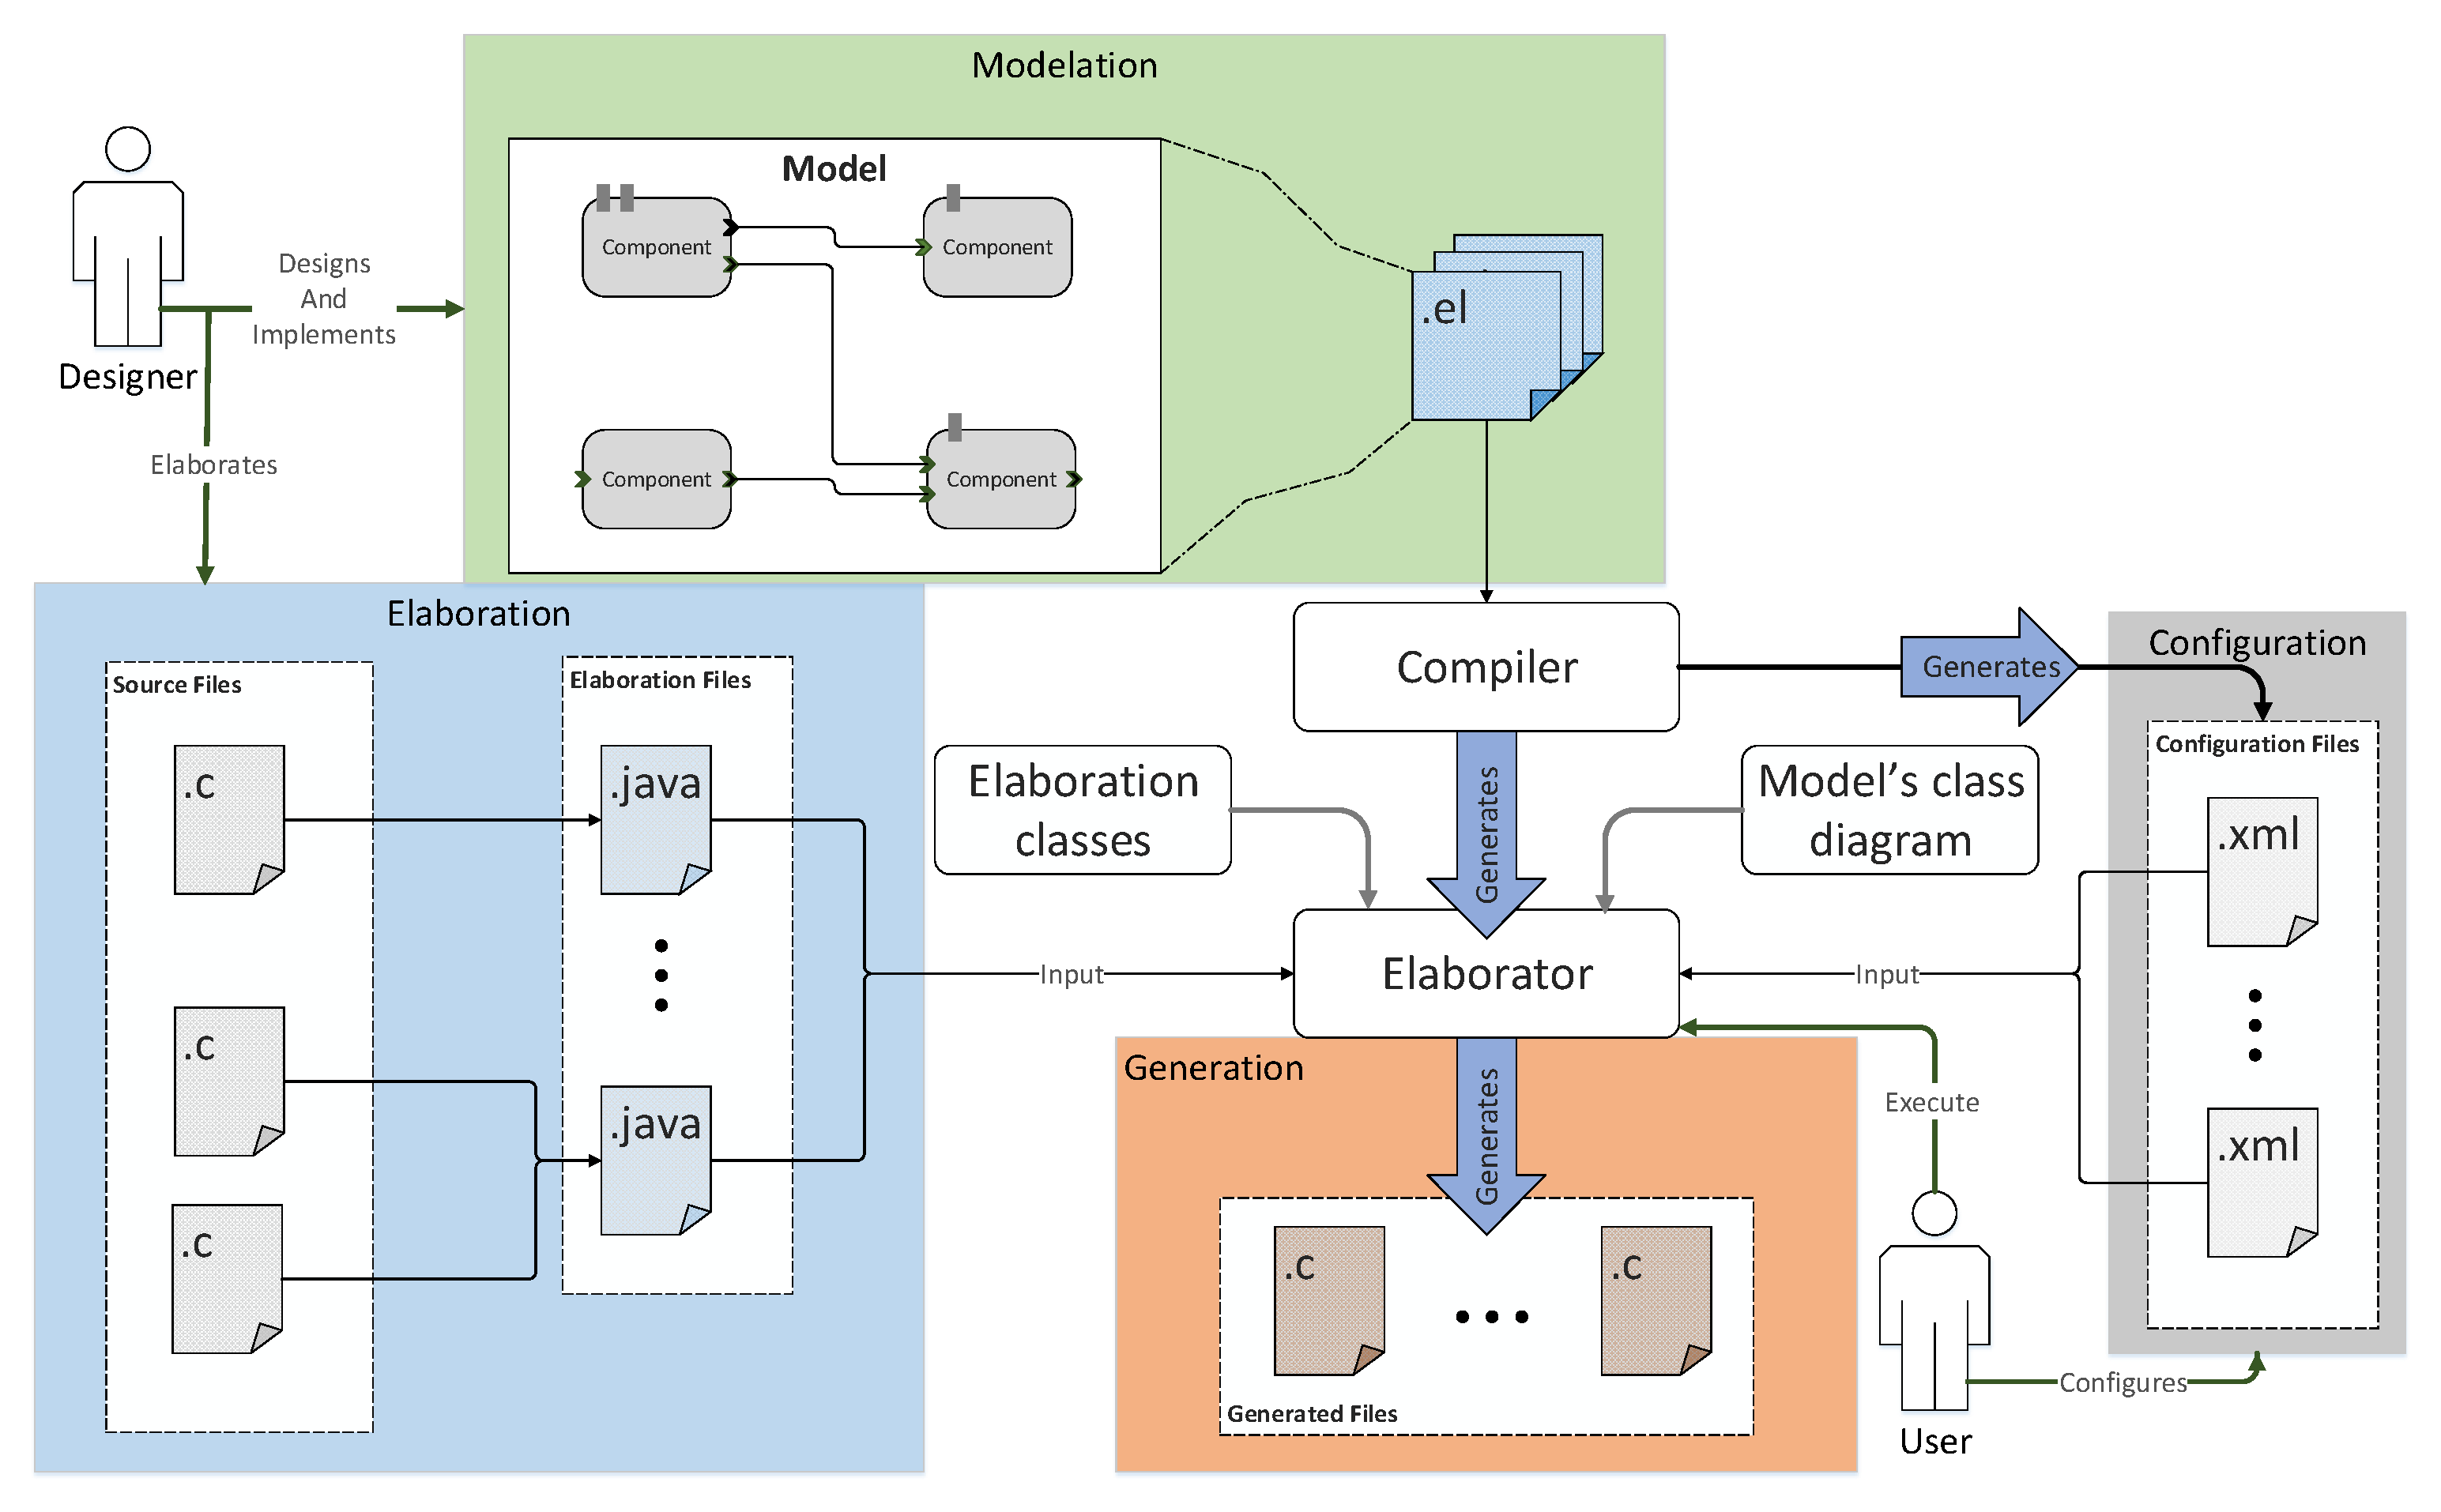
\includegraphics[scale=0.3]{images/EL_workflow} }
\caption{EL framework workflow.}
\label{fig:workflow} 
\end{figure}



\subsubsection{Final File System}

As it was explained in the \textit{Workflow} section, after the compilation of the \textit{.el} files, a several number of other files are generated. For organizational purposes,  folders are also generated and the files are stored inside of each folder respectively. Figure \ref{fig:file_system} illustrates the generated files system of the simple example that as been followed.   


Only some of the sub-folders of the file system are shown in the figure, the more relevant ones. It is possible to see the folders chain of the \textit{Configs} folder. It contains all the configuration files of each component of the model. Is in the \textit{Final Files} folder that will be stored the final source files, after the Elaborator operation. As for the \textit{SpecificElaborations} it is created a folder to each component and, inside of it, must be created folders to store the specific elaboration files along with the annotated sources. If an annotated source file will be manipulated by different elaborations files, that source must be stored in the \textit{SharedSources} folder.

\begin{figure}[H]
\centering
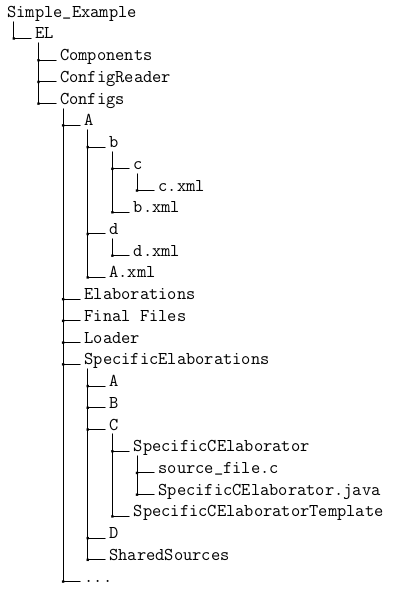
\includegraphics[scale=0.6]{images/files_system}
\caption{Final Files System.}
\label{fig:file_system} 
\end{figure}


